% $Id: gui_disres.tex 395 2011-11-17 22:34:59Z cphillip $
%
% Written by J. Schrouff for v2.0
%_______________________________________________


\chapter{Display voxel and region contribution}
\label{chap:DisWeights}
\minitoc

\section{Introduction}

Another important aspect of pattern recognition modelling when applied to neuroimaging is trying to interpret the models' parameters or weights. Some brain 
areas are probably more informative about class membership/regression targets than others. For example, in a visual
task, we would expect discriminative information in the occipital lobe. This can be seen as \textit{information mapping}, and it can be helpful to evaluate a specific model - if
the discriminative weight of a machine is concentrated in the eyes, for example, it is important
to correct the mask used in the analysis to exclude them. In the case of linear kernels, the classifier/regression weight
vector is a linear combination or weighted average of the training examples, and can be plotted
as an image representing a weight map. The \textit{weight map} is therefore a spatial representation
of the decision function, i.e. every voxel within the mask contributes with a certain weight to the decision function. 
Pattern recognition models (classifiers or regression functions) are multivariate, i.e. they
take into account correlations in the data. Since the discrimination or prediction is
based on the whole brain pattern, rather than on individual regions or voxels, all voxels
contribute to the classification or regression and no conclusions should be drawn about a particular
subset of voxels in isolation.

Starting from PRoNTo v2.0, it is possible to derive weights at the region level (as anatomically defined by an atlas, from MKL or from summarizing the weights). This window allows to display maps of voxel and of region contribution. Furthermore, the region contributions can be ranked in descending order, yielding a sorted list of regions according to their contribution to the classification/regression model. We hope this will help the interpretation of model parameters in terms of cognitive neuroscience.

\textbf{Important note:} The implemented version of MKL (\cite{Rakotomamonjy2008}) is sparse in the kernel combination. This means that only a few regions/modalities will contribute to the model. However, this selection of regions/modalities might depend on the dataset, and small variations in the dataset (as induced by cross-validation) might lead to different subsets of regions/modalities begin selected. Therefore, care should be taken when reporting selected regions/modalities and each fold should be looked at separately. We also provide a quantification of the variability across folds of the ranking of the regions/modalities (`Expected Ranking', see further) to provide some insights on this issue.


\section{Displaying weights}

To launch the `Display weights' window, make sure that weight maps have been computed for at least one model (Compute Weights, Chapter~\ref{chap:ComputeWeights}).

In the {\tt Review Options} panel, press {\tt Display weights}. At the `Select PRT.mat' window,
navigate to where your {\tt PRT.mat} file is stored (using the left column), and select it in the
right column. The display window then opens (Figure \ref{fig_prt_ui_weights_empty}).

\begin{figure}[h!]
\begin{center}
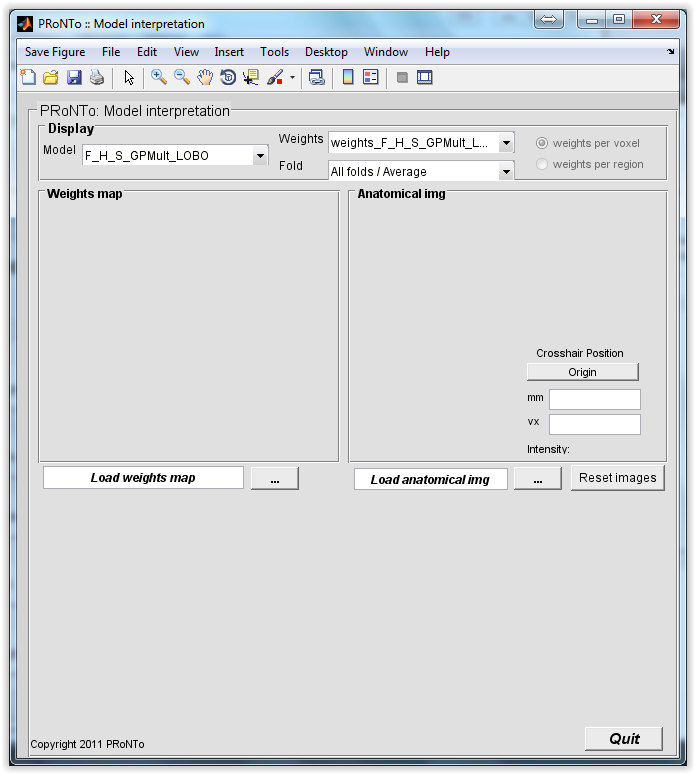
\includegraphics[height=9cm]{images/prt_ui_weights_empty.PNG}
\caption{Display weights main window after selection of PRT.mat.}
\label{fig_prt_ui_weights_empty}
\end{center}
\end{figure}


The window is divided into four panels; going from top left to bottom left, they
are:
\begin{description}
\item[Display]: This panel allows the user to choose which model and image to display, as well as whether to display the voxel weights or the region contributions.
\item[Weights map]: This displays three projections of the selected weight map and allows to navigate it.
\item[Anatomical img]: If an anatomical image has been loaded, this will display three projections,
and the cross-hair will be synchronised with the weight map.
\item[Additional plots]: The blank area at the bottom of the window will display additional information about the model parameters, such as a sorted list of the regions according to their contribution (if weights per region were computed, in the form of a table) and a bar plot of the relative region contribution. If MKL modelling was performed based on multiple modalities, the same table and bar plot will display the relative contributions of each modality to the decision function. 
\end{description}

\subsection{Select image to display}

The \texttt{Display} panel shows the models for which weights were computed and weight images were found in the same folder as the PRT. For each model, the list of images available is displayed in the \texttt{Weights} pop-down list. Typically, one image will be created for a binary comparison or regression with only one modality or multiple modalities concatenated in samples (e.g. multiple runs). On the other hand, multiclass classification models will return one image per class (with the index of the class appended to the name of the image). In the same way, multiple modalities used in multiple kernels will lead to the building of \textit{number of modalities} images. For each image, the weight map can be displayed for each fold or for their average. In PRoNTo v2.0, it is possible to display the contributions of each voxel (\texttt{weights per voxel}) or of each region (\texttt{weights per region}, if previously computed).

\textbf{Note:} the weight images (per voxel and per region) are automatically detected in the list of files in the PRT folder according to the name specified in the `Compute weights' step (Chapter \ref{chap:ComputeWeights}). Modifying the image name afterwards or moving the images might lead to warning messages and the images will not be listed in the GUI.

To display a weight image, select a model, an image and a fold. If only weights per voxel were estimated, the window will look similar to Figure \ref{fig_prt_ui_weights_img}.

\begin{figure}[h!]
\begin{center}
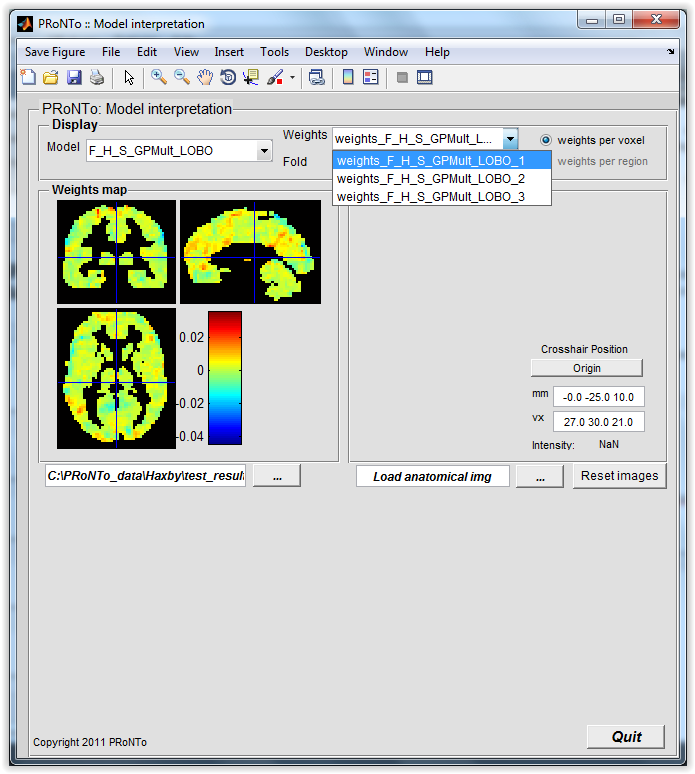
\includegraphics[height=9cm]{images/prt_ui_weights_img.PNG}
\caption{Displaying weight image for class 1 of a three-class GP model (Haxby dataset).}
\label{fig_prt_ui_weights_img}
\end{center}
\end{figure}

\subsection{Weights map}

The weight map is displayed with a cross-hair and a colorbar. The colorbar indicates the
relative importance of the voxel in the decision function. This value is also
indicated in the {\tt intensity} field of the {\tt Anatomical img} panel. Note that all voxels
in the mask contribute to the decision function, since the analysis is multivariate. Contrary
to common practice in Statistical Parametric Mapping, which is a mass-univariate approach, {\em it does
not make sense to isolate part of the pattern and report only on the peaks of the distribution
of the decision function's weight map, unless they have perfectly null contribution (as might happen with sparse models such as L1-MKL modelling)}. 

Below the displayed image, an edit box and a `browse' ($[${\tt ...}$]$) button also allow to load a weight image (.img) that is not linked to a model (e.g. from a previous PRoNTo version).

\subsection{Anatomical image}

By clicking on the $[${\tt ...}$]$ button next to the {\tt Load anatomical img} field, 
a dialogue opens that allows you to select an anatomical images {\tt .img} file that was co-registered with the data images.

In this panel, the cross-hair position is displayed in voxels and in mm. It can also be reset to the origin of the image. For each position, the corresponding voxel weight is displayed in the `intensity' field.

\subsection{Additional plots}

Additional information will be displayed in two main cases:
\begin{itemize}
\item \textbf{Multiple Kernel Learning modelling:} MKL modelling, based on modalities or on regions as defined by an atlas, will provide weights at two levels: the kernel level and the voxel level. The kernel contributions, which sum to 1, can then be ranked in descending order. 
\item \textbf{Summarizing weights per region:} in PRoNTo v2.0, weights can be summarized within regions of interest as defined by an atlas (user-specified). For each region, a normalized contribution can be defined, and those contributions can then be ranked in descending order. 
\end{itemize}

In both cases, the region/modality contributions will be displayed in a table as well as in a bar plot, for each fold and for their average (according to the selected fold in the \texttt{Display} panel). An example is displayed in Figure \ref{fig_prt_ui_weights_ROI}, for weight summarization after GP modelling.

\begin{figure}[h!]
\begin{center}
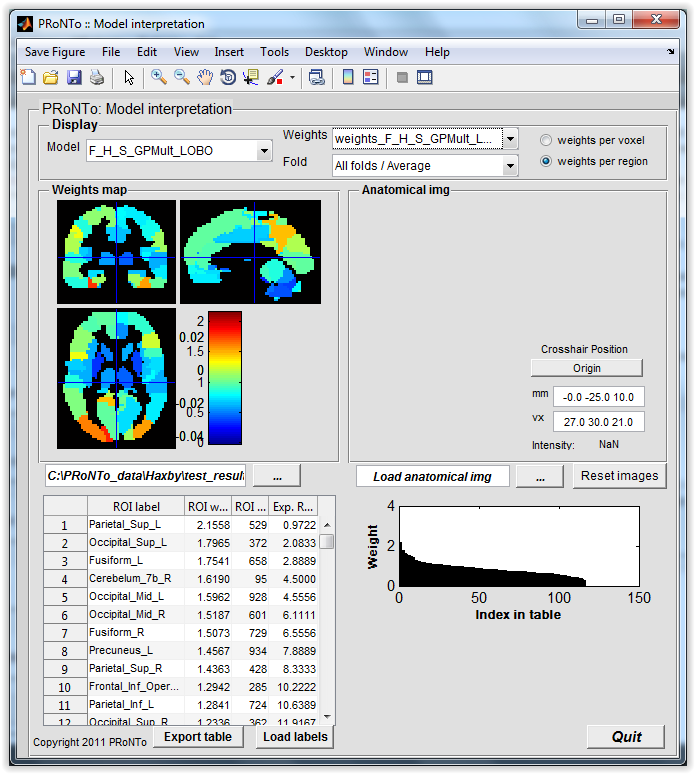
\includegraphics[height=9cm]{images/prt_ui_weights_ROI.PNG}
\caption{Displaying ROI contributions for class 1 of a three-class GP model (Haxby dataset).}
\label{fig_prt_ui_weights_ROI}
\end{center}
\end{figure}

In the case where kernels were built both at the modality and at the region level (i.e. multiple modalities with each multiple regions as defined by an atlas), two tables will be displayed (one for regions, one for modalities). The table for modalities will sum the contributions of each region within that modality.

\subsubsection{Sorted table of region/modality contributions}

The displayed table comprises one row per region and 5 columns (for an example on ROIs, as displayed in Figure \ref{fig_prt_ui_weights_ROI}):

\begin{itemize}
\item \textbf{Index of the ROI:} The first column displays the ranking of the region of interest in the selected fold, according to its contribution.
\item \textbf{ROI Label:} When using the atlas provided in \textit{your PRoNTo folder/atlas}, the labels of each region will be loaded automatically from a .mat, stored alongside the atlas. If using another atlas, the labels can be loaded through the `Load Labels' button. In this case, the user should select a .mat comprising a cell array of size \textit(number of regions,1), with the label for each region in the corresponding cell (in characters). The cell array should be saved under the variable name `ROI\_ names'. Otherwise, generic names will be used (e.g. ROI\_ 1).
\item \textbf{ROI weight:} The (normalized) contribution of each region is displayed in the third column (in \%). The rows of the table are sorted in descending order according to this value. 
\item \textbf{ROI size:} This column displays the size of the ROI in voxels. This gives indications on the overlap between the atlas and the data.
\item \textbf{Expected Ranking}: This measure reflects how stable the ranking of the region is across folds. It is computed from the ranking in each fold (see \cite{Schrouff2013a} for details), and is therefore the same, whether the user is displaying fold 1, or the average of all folds. If the Expected Ranking (ER) is close to the ranking in the selected fold, then it reflects that this region has a similar ranking across folds. On the contrary, if the ER is quite different from the ranking shown for the selected fold, this means that the ranking might be variable across folds. This variability can come from the fact that the region did not have the same contribution to slightly different datasets. It might also happen that it is not selected at all in some folds (as can happen with L1-MKL since it will not select kernels with correlated information).
\end{itemize}

When selecting a specific region label in the table, the weight map will only display colored voxel or region weights (according to which plot was selected) for this region, the rest of the image being in grey scale. This allows e.g. to look closely at the voxel weights within a region that highly contributes to the selected model and fold (Figure \ref{fig_prt_ui_weights_specROI}).

\begin{figure}[h!]
\begin{center}
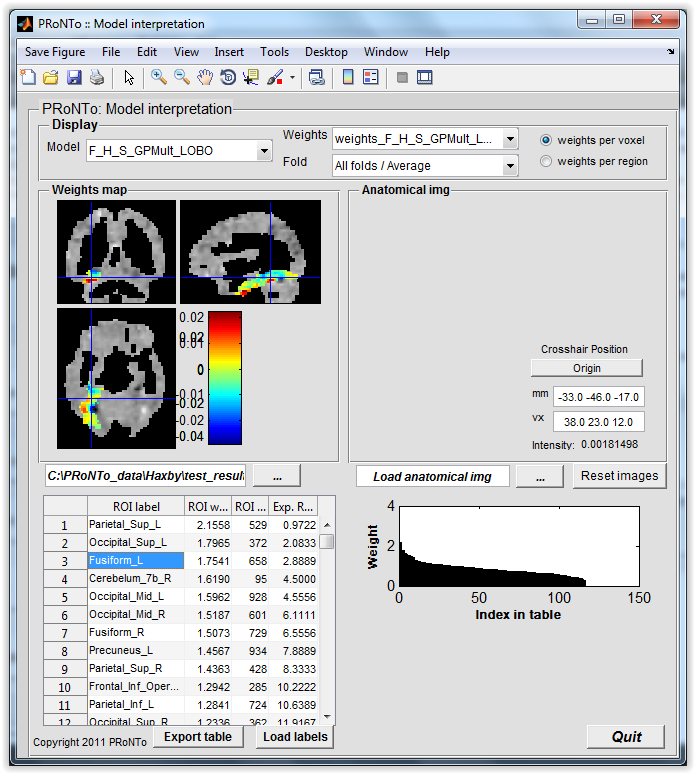
\includegraphics[height=9cm]{images/prt_ui_weights_specROI.PNG}
\caption{Displaying fusiform weights for binary MKL model (Haxby data).}
\label{fig_prt_ui_weights_specROI}
\end{center}
\end{figure}


Finally, the table can be exported as a text file using the `Export Table' button.

\subsubsection{Bar plot of contributions}
The bar plot displays the third column of the table, i.e. the contribution of each ROI or modality to the decision function. The x-axis represents the index of the ROI in the table (i.e. first column of the table), in the selected fold, while the y-axis displays the contribution of each region/modality. The bar graph provides insights on how sparse or dense the region/modality contributions are.




